%xelatex
\documentclass{article}
\usepackage[margin=0.6in]{geometry}
\usepackage{xltxtra}
\usepackage{xgreek}
\usepackage{listings}
\setmainfont[Mapping=tex-text]{Kerkis}
\usepackage[colorlinks=true,linkcolor=black,urlcolor=blue]{hyperref}
\title{Παράλληλη επεξεργασία}
\author{Μπαντολας Πέτρος 5028\\Σειμένης Σπύρος 5070\\Καλλιβωκάς Δημήτριος 4993}

\lstset{columns=flexible}
\lstset{keepspaces=true}

\begin{document}
\maketitle
\section{Ανάλυση σειριακής έκδοσης}

\begin{center}
\begin{tabular}{|r|l|}
    \hline
    Επίπεδο Βελτιστοποίησης & Χρόνος Εκτέλεσης \\ \hline
    O0 & 77.5 sec \\
    O3 & 27.91 sec \\ \hline
\end{tabular}
\end{center}

Η συμπεριφορά της σειριακής εκδοσης έγινε με την χρήση του εργαλείου scalasca.
\begin{center}
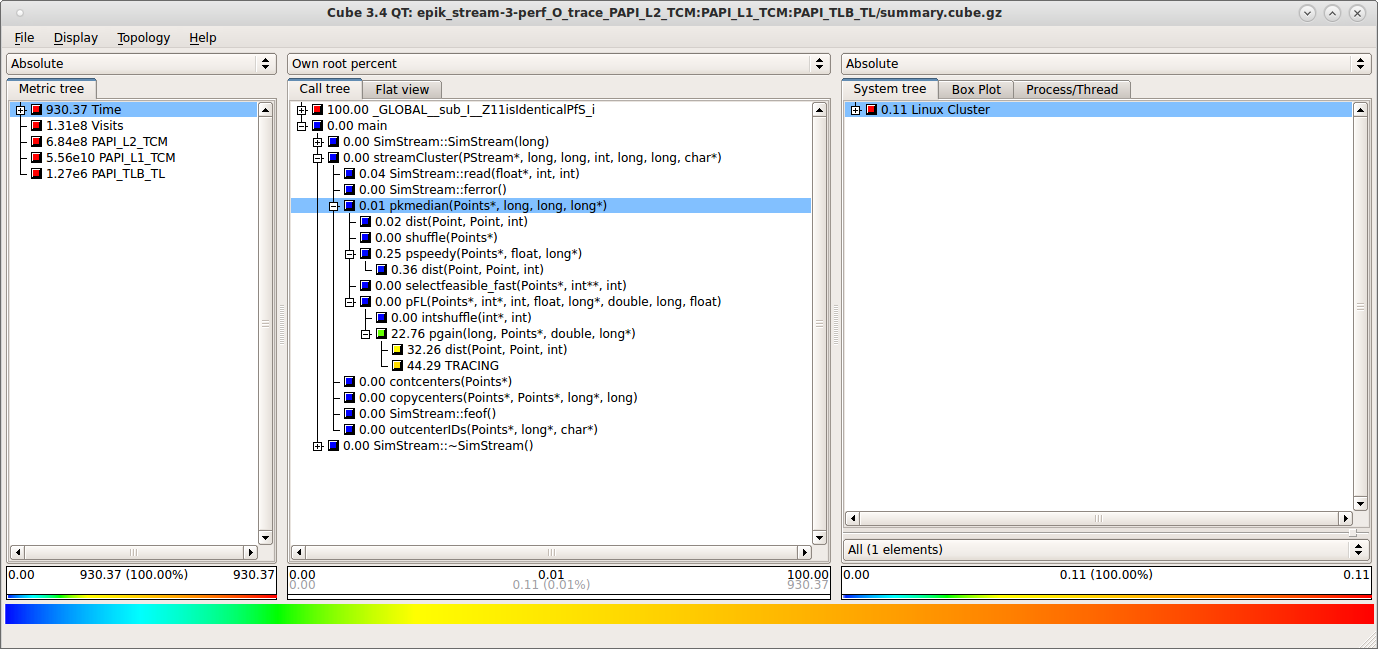
\includegraphics[scale=0.5]{../scrshots/time.png}
\end{center} 
Όπως φαινεται και στην εικόνα, οι συναρτήσεις με τον μεγαλύτερο χρόνο εκτέλεσης ειναι η pspeedy και η pgain.\\
Συγκεκριμένα ο μεγαλύτερος χρόνος και των δύο είναι κατα τις κλήσεις τους στην συνάρτηση dist.
\subsection{pgain}
Παρακάτω φαίνονται τα L1, L2, TLB cache misses της σειριακής έκδοσης όπου επι το πλείστον οφείλονται στην pgain.
\begin{center}
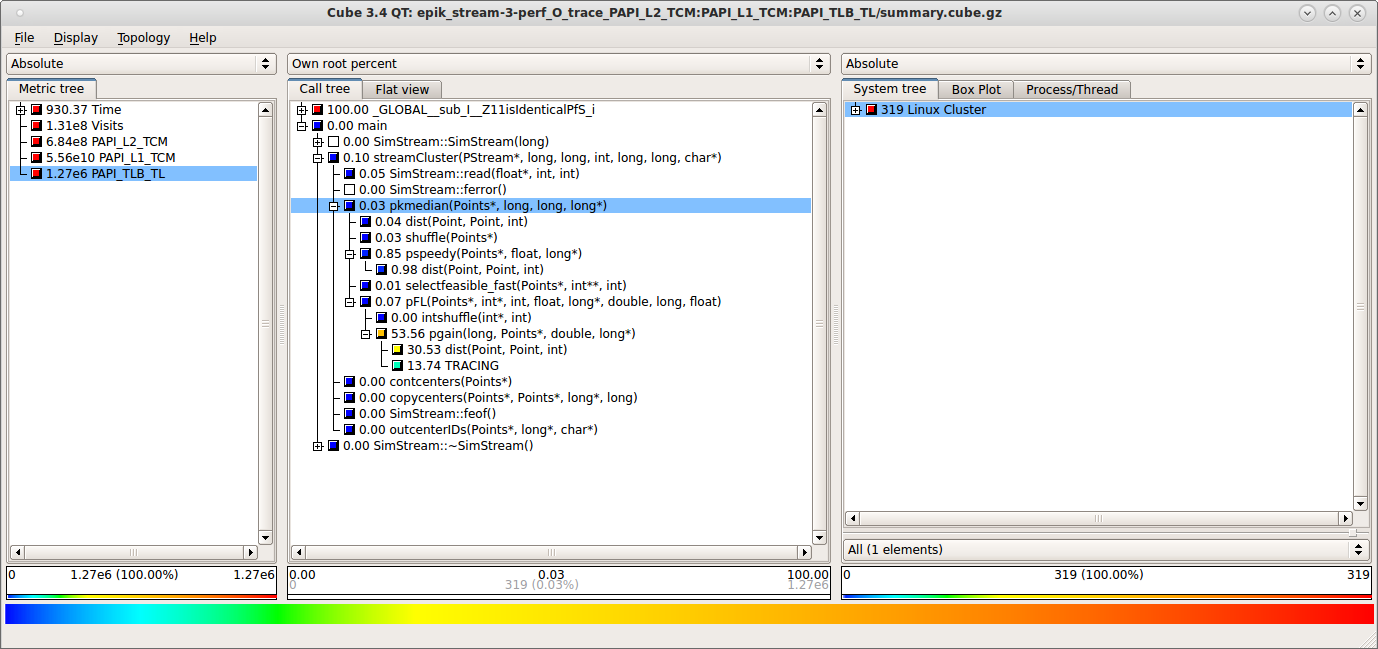
\includegraphics[scale=0.4]{../scrshots/tlb.png}
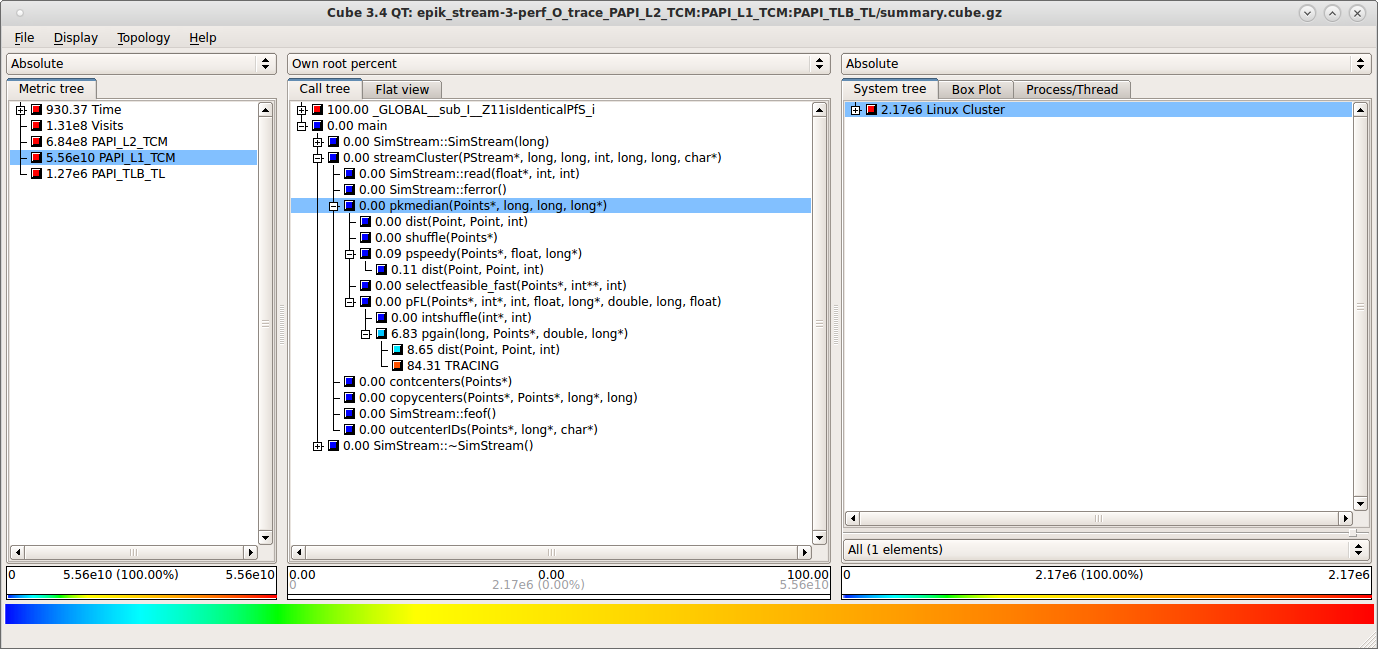
\includegraphics[scale=0.4]{../scrshots/l1.png}
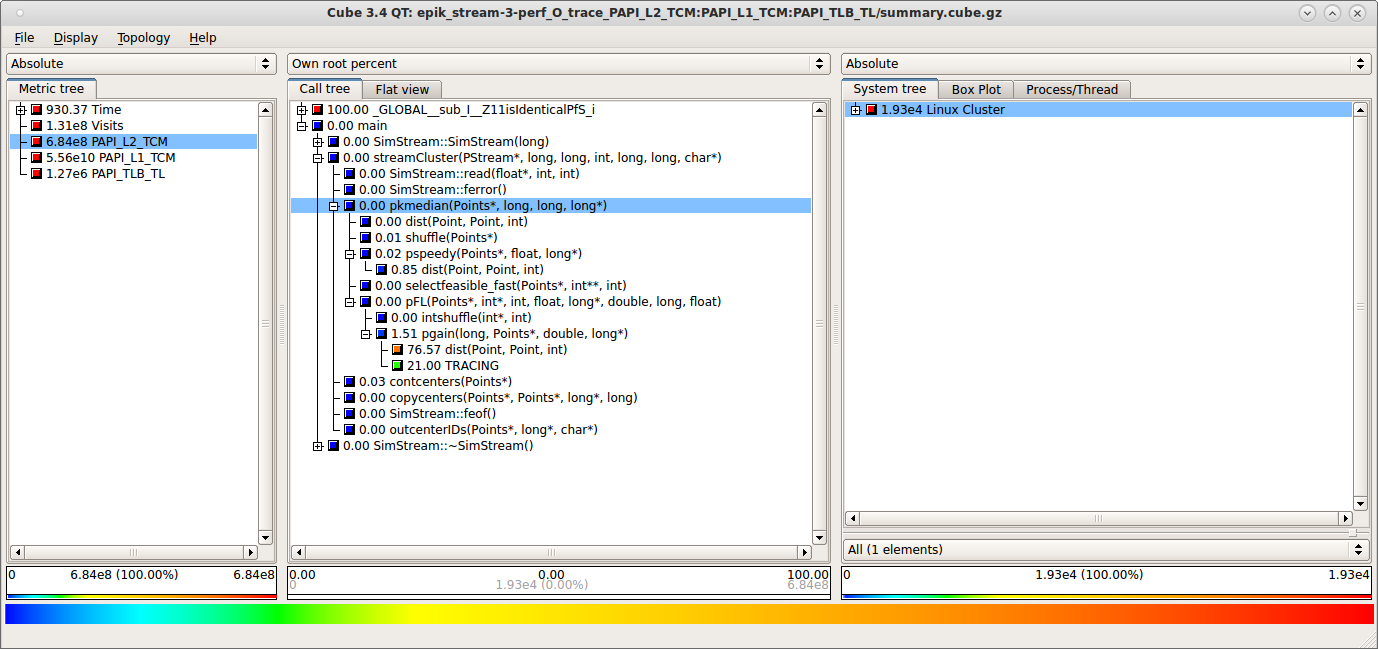
\includegraphics[scale=0.4]{../scrshots/l2.png}
\end{center} 
Συμπεραίνουμε οτι οι περιοχές που προκαλούν καθυστέρηση είναι αυτές που υπολογίζουν κατ' επανάληψη για όλα τα σημεία την απόσταση τους(dist). Αυτό γίνεται για ολα τα σημεία άρα για μεγάλο αριθμό σημείων αυξάνεται και η πολυπλοκοτητα του προγράμματος. Επίσης η δομή που αποθηκεύει τα σημεία δεσμεύεται στην αρχή του προγράμματος στο heap μεσω malloc που δεν εγγυάται ότι οι διευθύνσεις φυσικής μνήμης θα είναι γειτονικες μεταξυ τους. Η πολλαπλή προσπέλαση όλων των σημείων σειριακά οδηγεί στα
πολλαπλά cache misses. Έτσι η παραλληλοποίηση με openmp βελτιστοποιεί τους υπολογισμούς μειώνοντας τα cache misses.

\section{Χρονοβελτίωση}
\subsection{Με χρήση OpenMP}
Σύμφωνα με την προηγούμενη ανάλυση, τα σημεία όπου χρειάζεται χρονοβελτίωση είναι κυρίως οι κλήσεις της \texttt{dist} μέσα στις συναρτήσεις \texttt{pgain} και \texttt{pspeedy}.

Δύο είναι τα σημεία μέσα στην \texttt{pgain} όπου καλείται σε βρόχο \texttt{for} η \texttt{dist}. Εισάγοντας εκεί εντολές \texttt{OpenMP} μειώνεται αρκετά ο χρόνος εκτέλεσης.
\begin{lstlisting}
#pragma omp parallel for \
shared(switch_membership,points,lower,center_table,x) private(i) \
reduction(+:cost_of_opening_x) \
schedule(static)
for ( i = 0; i < points->num; i++ ) {
    float x_cost = dist ( points->p[i], points->p[x], points->dim ) * points->p[i].weight;
    float current_cost = points->p[i].cost;
\end{lstlisting}
Εδώ απαιτείται reduction για την μεταβλητή \texttt{cost\_of\_opening\_x} αφού είναι κοινή σε όλα τα νήματα.

\begin{lstlisting}
int assign = points->p[i].assign;
#pragma omp atomic
lower[center_table[assign]] += current_cost - x_cost;
\end{lstlisting}
Η εντολή atomic απαιτείται για να αποκλειστούν ενημερώσεις στην ίδια θέση του πίνακα \texttt{lower} απο διαφορετικά νήματα.

\begin{lstlisting}
#pragma omp parallel for \
shared(points,gl_lower,center_table,switch_membership,x) \
schedule(static)
for ( int i = 0; i < points->num; i++ ) {
    bool close_center = gl_lower[center_table[points->p[i].assign]] > 0 ;
    if ( switch_membership[i] || close_center ) {
\end{lstlisting}

Ακόμη, στη συνάρτηση \texttt{pspeedy} καλείται σε ένθετο βρόχο η \texttt{dist}. Εισάγοντας σε αυτό το σημείο παραλληλοποίηση με \texttt{OpenMP} παρατηρείται μια μικρή βελτίωση στο χρόνο.

\begin{lstlisting}
#pragma omp parallel for \
shared(points) \
schedule(static)
for ( int k = 0; k < points->num; k++ )  {
    float distance = dist ( points->p[i],points->p[k],points->dim );
\end{lstlisting}

Σε όλες τις παραπάνω περιπτώσεις επιλέχθηκε στατικός διαμοιρασμός των επαναλήψεων στα νήματα, αφού ο φόρτος είναι ο ίδιος σε κάθε περίπτωση (καλείται η συνάρτηση \texttt{dist} με σταθερό πλήθος σημείων).

\begin{center}
\begin{tabular}{|r|c|c|}
    \hline
    Νήματα & Χρόνος Εκτέλεσης (-Ο0) & Χρόνος Εκτέλεσης (-Ο3) \\ \hline
    1 & 79.8 sec & 28.4 sec \\
    2 & 43.1 sec & 16.2 sec \\
    4 & 26.2 sec & 12.4 sec \\ \hline
\end{tabular}
\end{center}

\subsection{Με χρήση εντολών SIMD}
Λαμβάνοντας υπόψη την ανάλυση της σειριακής έκδοσης του προγράμματος και οι δύο συναρτήσεις σπαταλούν τον μεγαλύτερο χρόνο στην συνάρτηση dist η οποία υπολογίζει την απόσταση δυο σημείων πολλαπλών διαστάσεων.\\
Ο χρόνος στον οποίο η dist υπολογίζει την απόσταση δυο σημείων μπορεί να βελτιωθεί χρησιμοποιώντας εντολές simd.\\
Αρχικά υπολογίζονταν η διαφορά μεταξύ των δύο σημείων σειριακά για κάθε διάστασή τους. Πλέον οι τιμές κάθε διάστασης των σημείων φορτώνονται ανα 4 ως διάνυσμα σε καταχωρητές των 128 bit του επεξεργαστή, οι αφαιρέσεις και πολλαπλασιασμοί που χρειάζονται γίνονται ανά 4 και έτσι επιταχύνεται η διαδικασία.

\begin{center}
\begin{tabular}{|r|c|c|}
    \hline
    Νήματα & Χρόνος Εκτέλεσης (-O0) & Χρόνος Εκτέλεσης (-Ο3) \\ \hline
    1 & 102.6 sec & 18.2 sec \\
    2 & 54.8 sec & 12.2 sec \\
    4 & 29.0 sec & 14.0 sec \\ \hline
\end{tabular}
\end{center}

\section{Συμπεράσματα}
Στο παρακάτω διάγραμμα απεικονίζεται συνοπτικά η χρονοβελτίωση των παραπάνω υλοποιήσεων.
\begin{center}
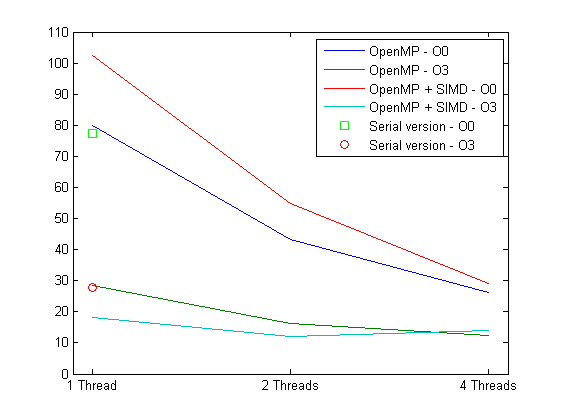
\includegraphics{../scrshots/results.png}
\end{center} 

Παρατηρείται ότι στις περιπτώσεις χωρίς βελτιστοποίηση η έκδοση με SIMD είναι πιο αργή σε σχέση με την έκδοση μόνο με openmp. Αν και δεν φαίνεται λογικό εκ πρώτης όψεως, η χειρότερη απόδοση του simd οφείλεται στο ότι έχουν αφαιρεθεί οι βελτιστοποιήσεις του compiler. Σε πραγματικές συνθήκες δεν θα συνέβαινε ποτέ αυτό.\\\\
Όταν οι βελτιστοποιήσεις του compiler είναι ενεργές, προσθέτοντας simd εντολές στην έκδοση με openMP επιτυγχάνεται περαιτέρω μείωση του χρόνου.\\

\end{document}
